\chapter{Seleksi, Hanyutan dan Spesiasi}\label{ch:g12:selection-drift-speciation}

Pada 1848 sebuah bentuk hitam ngengat lada tertangkap di dekat sebuah
kota industri yang setiap batang pohonnya berlapis jelaga; pada 1895
hampir semua ngengat di wilayah itu berwarna hitam. Seabad kemudian,
dengan jelaga yang lenyap dan batang yang kembali pucat, bentuk hitam
itu nyaris menghilang. Tidak ada yang membiakkan ngengat itu; burung
pemakannyalah yang melakukan penyortiran. Dua bab terakhir menjelaskan
bagaimana keragaman muncul; bab ini tentang apa yang terjadi padanya di
dalam sebuah \omterm{def:g12:selection-drift-speciation:population}{populasi} --- bagaimana sebagian \omterm{def:g10:universal-dna:gene}{alel} menjadi umum dan
sebagian lain menjadi jarang, oleh seleksi dan oleh kebetulan --- dan
bagaimana, pada akhirnya, satu \omterm{def:g12:selection-drift-speciation:population}{populasi} menjadi dua \omterm{def:g10:biodiversity-scales:species}{spesies}.

\section{Populasi dan alelnya}

\begin{definition}[Populasi, frekuensi alel]\label{def:g12:selection-drift-speciation:population}
Sebuah \emph{populasi}\index{populasi} adalah himpunan individu satu
\omterm{def:g10:biodiversity-scales:species}{spesies} yang hidup di tempat yang sama dan berbiak di antara mereka
sendiri. Susunan genetiknya digambarkan oleh
\emph{frekuensi}\index{frekuensi alel} \omterm{def:g10:universal-dna:gene}{alel} setiap \omterm{def:g10:universal-dna:gene}{gen}: untuk sebuah
\omterm{def:g10:universal-dna:gene}{gen} dengan dua \omterm{def:g10:universal-dna:gene}{alel} $A$ dan $a$, yaitu bagian $p$ dari semua salinan
yang berupa $A$ dan bagian $q = 1 - p$ yang berupa $a$. Evolusi, pada
skala ini, adalah perubahan frekuensi \omterm{def:g10:universal-dna:gene}{alel} dari satu generasi ke
generasi berikutnya.
\end{definition}

\begin{proposition}[Frekuensi tanpa gaya apa pun]\label{prop:g12:selection-drift-speciation:hw}
Dalam \omterm{def:g12:selection-drift-speciation:population}{populasi} besar yang perkawinannya acak, yang tidak ada \omterm{def:g10:universal-dna:gene}{alelnya}
memberi keuntungan, dan yang tidak mengalami \omterm{def:g11:mutations:mutation}{mutasi} atau migrasi,
\omterm{def:g12:selection-drift-speciation:population}{frekuensi alel} tetap sama dari generasi ke generasi, dan \omterm{def:g11:enzymes-and-phenotype:phenotype}{genotipe}
muncul dalam perbandingan
\[
AA : Aa : aa = p^2 : 2pq : q^2 .
\]
Inilah keadaan acuan: setiap penyimpangan darinya, yang teramati
sepanjang generasi, adalah tanda bahwa salah satu syarat telah gagal
--- bahwa seleksi, kebetulan, migrasi atau \omterm{def:g11:mutations:mutation}{mutasi} sedang bekerja.
\end{proposition}
\begin{proof}
Setiap gamet membawa $A$ dengan peluang $p$ dan $a$ dengan peluang
$q$; dua gamet yang diambil acak memberi $AA$ dengan peluang $p^2$,
$aa$ dengan $q^2$, dan $Aa$ dengan $pq + qp = 2pq$. Mencacah \omterm{def:g10:universal-dna:gene}{alel}
generasi baru: salinan $A$ menyusun $p^2 + \tfrac12 (2pq) =
p(p + q) = p$ dari keseluruhan. Frekuensinya tidak berubah.
\end{proof}

\begin{omfigure}
\begin{tikzpicture}[font=\small]
  \draw[thick] (0,0) rectangle (5,5);
  \fill[omDef!25] (0,1.5) rectangle (3.5,5);
  \fill[omProp!25] (3.5,1.5) rectangle (5,5);
  \fill[omProp!25] (0,0) rectangle (3.5,1.5);
  \fill[omThm!30] (3.5,0) rectangle (5,1.5);
  \draw (3.5,0) -- (3.5,5); \draw (0,1.5) -- (5,1.5);
  \node at (1.75,3.25) {$AA$: $p^2$}; \node at (4.25,3.25) {$Aa$: $pq$};
  \node at (1.75,0.75) {$Aa$: $pq$}; \node at (4.25,0.75) {$aa$: $q^2$};
  \node[anchor=south] at (1.75,5.1) {$A$, frekuensi $p$}; \node[anchor=south] at (4.25,5.1) {$a$, $q$};
  \node[anchor=east] at (-0.1,3.25) {$A$, $p$}; \node[anchor=east] at (-0.1,0.75) {$a$, $q$};
  \node[anchor=south, font=\small\itshape] at (2.5,5.6) {gamet ayah};
  \node[font=\small\itshape, rotate=90, anchor=south] at (-1.1,2.5) {gamet ibu};
  \node[anchor=west, align=left, text width=6cm] at (6,2.5) {Dengan $p = 0.7$ dan $q = 0.3$: $AA$ 49\%, $Aa$ 42\%, $aa$ 9\%. Sifat resesif yang tampak pada 9\% populasi dibawa, tanpa terlihat, oleh 42\% lainnya.};
\end{tikzpicture}

{\small Perbandingan \omterm{def:g11:enzymes-and-phenotype:phenotype}{genotipe} perkawinan acak, sebagai luas. Sisi
persegi itu adalah frekuensi gamet; keempat persegi panjangnya adalah
\omterm{def:g11:enzymes-and-phenotype:phenotype}{genotipe}. Heterozigot memuat sebagian besar salinan \omterm{def:g10:universal-dna:gene}{alel} yang jarang.}
\end{omfigure}

\begin{example}[Mencacah alel]\label{ex:g12:selection-drift-speciation:count}
Di antara 1000 orang, 490 bergenotipe $AA$, 420 $Aa$ dan 90 $aa$. Salinan $a$:
$420 + 2 \times 90 = 600$ dari 2000, sehingga $q = 0.3$ dan $p = 0.7$ ---
dan cacah \omterm{def:g11:enzymes-and-phenotype:phenotype}{genotipenya} persis $p^2$, $2pq$, $q^2$ dari 1000: \omterm{def:g12:selection-drift-speciation:population}{populasi}
itu berada pada keadaan acuan untuk \omterm{def:g10:universal-dna:gene}{gen} ini. Penyakit \omterm{def:g11:genes-and-disease:genetic}{resesif} yang
menimpa satu bayi dari 2500 ($q^2 = 1/2500$) menyiratkan $q = 1/50$ dan
\omterm{def:g11:genes-and-disease:genetic}{pembawa} $2pq \approx 1/25$: angka-angka
\cref{ch:g11:genes-and-disease}, yang diturunkan.
\end{example}

\section{Seleksi}

\begin{definition}[Seleksi alam]\label{def:g12:selection-drift-speciation:selection}
\emph{Seleksi alam}\index{seleksi alam} adalah perbedaan reproduksi
antara individu yang membawa \omterm{def:g10:universal-dna:gene}{alel} berbeda, di dalam suatu lingkungan
tertentu: \omterm{def:g11:genes-and-disease:genetic}{pembawa} satu \omterm{def:g10:universal-dna:gene}{alel} meninggalkan, rata-rata, lebih banyak
keturunan daripada \omterm{def:g11:genes-and-disease:genetic}{pembawa} \omterm{def:g10:universal-dna:gene}{alel} lain, dan \omterm{def:g12:selection-drift-speciation:population}{frekuensi alel} itu naik dari
generasi ke generasi. Yang terseleksi adalah individu seutuhnya ---
kelangsungan hidupnya, perkawinannya, kesuburannya --- dan \omterm{def:g10:universal-dna:gene}{alelnya}
sekadar ikut terbawa.
\end{definition}

\begin{proposition}[Seleksi mengubah frekuensi ke satu arah]\label{prop:g12:selection-drift-speciation:direction}
\omterm{def:g10:universal-dna:gene}{Alel} yang \omterm{def:g11:genes-and-disease:genetic}{pembawanya} berhasil bereproduksi sedikit saja lebih baik
akan menyebar; \omterm{def:g10:universal-dna:gene}{alel} yang \omterm{def:g11:genes-and-disease:genetic}{pembawanya} kurang berhasil menjadi jarang.
Arahnya ditentukan oleh lingkungan, dan berbalik jika lingkungan
berbalik; lajunya bergantung pada besar keuntungan dan pada apakah \omterm{def:g10:universal-dna:gene}{alel}
itu terungkap dalam satu salinan (\omterm{def:g11:genes-and-disease:genetic}{dominan}, cepat) atau hanya dalam dua
(\omterm{def:g11:genes-and-disease:genetic}{resesif}, mula-mula lambat, dan tidak pernah benar-benar lenyap, sebab
salinannya yang jarang bersembunyi di dalam heterozigot).
\end{proposition}
\begin{proof}[Bukti percobaan]
Ngengat lada: burung memangsa ngengat yang terlihat; pada batang
berjelaga bentuk pucatlah yang terlihat, pada batang bersih bentuk
gelap; \omterm{def:g12:selection-drift-speciation:population}{frekuensi alel} gelap naik dari nyaris nol ke 98\% dalam lima
puluh tahun pencemaran dan turun kembali di bawah 10\% dalam empat
puluh tahun udara bersih, mengikuti batang pohonnya. Resistansi
\omterm{def:g11:antibiotic-resistance:antibiotic}{antibiotik} (\cref{ch:g11:antibiotic-resistance}): hanya \omterm{def:g11:genes-and-disease:genetic}{pembawa} \omterm{def:g10:universal-dna:gene}{alel}
resistan yang bereproduksi ketika obat hadir. Persistensi laktase
(\cref{ch:g11:enzymes-and-phenotype}): \omterm{def:g10:universal-dna:gene}{alel} itu umum justru di tempat
susu telah menjadi makanan orang dewasa selama ribuan tahun. Dalam
setiap kasus, nasib \omterm{def:g10:universal-dna:gene}{alel} mengikuti lingkungannya.
\end{proof}

\begin{omfigure}
\begin{tikzpicture}
\begin{axis}[
  width=0.88\linewidth, height=5.6cm,
  axis x line=bottom, axis y line=left,
  xmin=1840, xmax=2000, ymin=0, ymax=110,
  xlabel={tahun}, ylabel={ngengat gelap (\% tangkapan)},
  xlabel style={font=\small, at={(axis description cs:0.5,-0.12)}, anchor=north},
  ylabel style={font=\small},
  tick label style={font=\small}, xtick={1850,1875,1900,1925,1950,1975,2000}, ytick={0,25,50,75,100},
  clip=false,
]
\addplot[thick, omThm, mark=*, mark size=1.3pt] coordinates
  {(1848,1) (1860,10) (1870,40) (1880,75) (1895,98) (1920,97) (1950,95) (1960,90) (1970,60) (1980,30) (1990,10) (1998,4)};
\draw[dashed, gray] (axis cs:1956,0) -- (axis cs:1956,105);
\node[font=\scriptsize, anchor=south] at (axis cs:1956,105) {undang-undang udara bersih};
\end{axis}
\end{tikzpicture}

{\small Frekuensi bentuk gelap ngengat lada di dekat sebuah kota
industri (dibulatkan dari koleksi museum dan hasil tangkapan).
Kenaikannya mengikuti menghitamnya batang pohon; penurunannya,
pembersihannya. Seleksi berbalik ketika lingkungan berbalik.}
\end{omfigure}

\begin{omfigure}
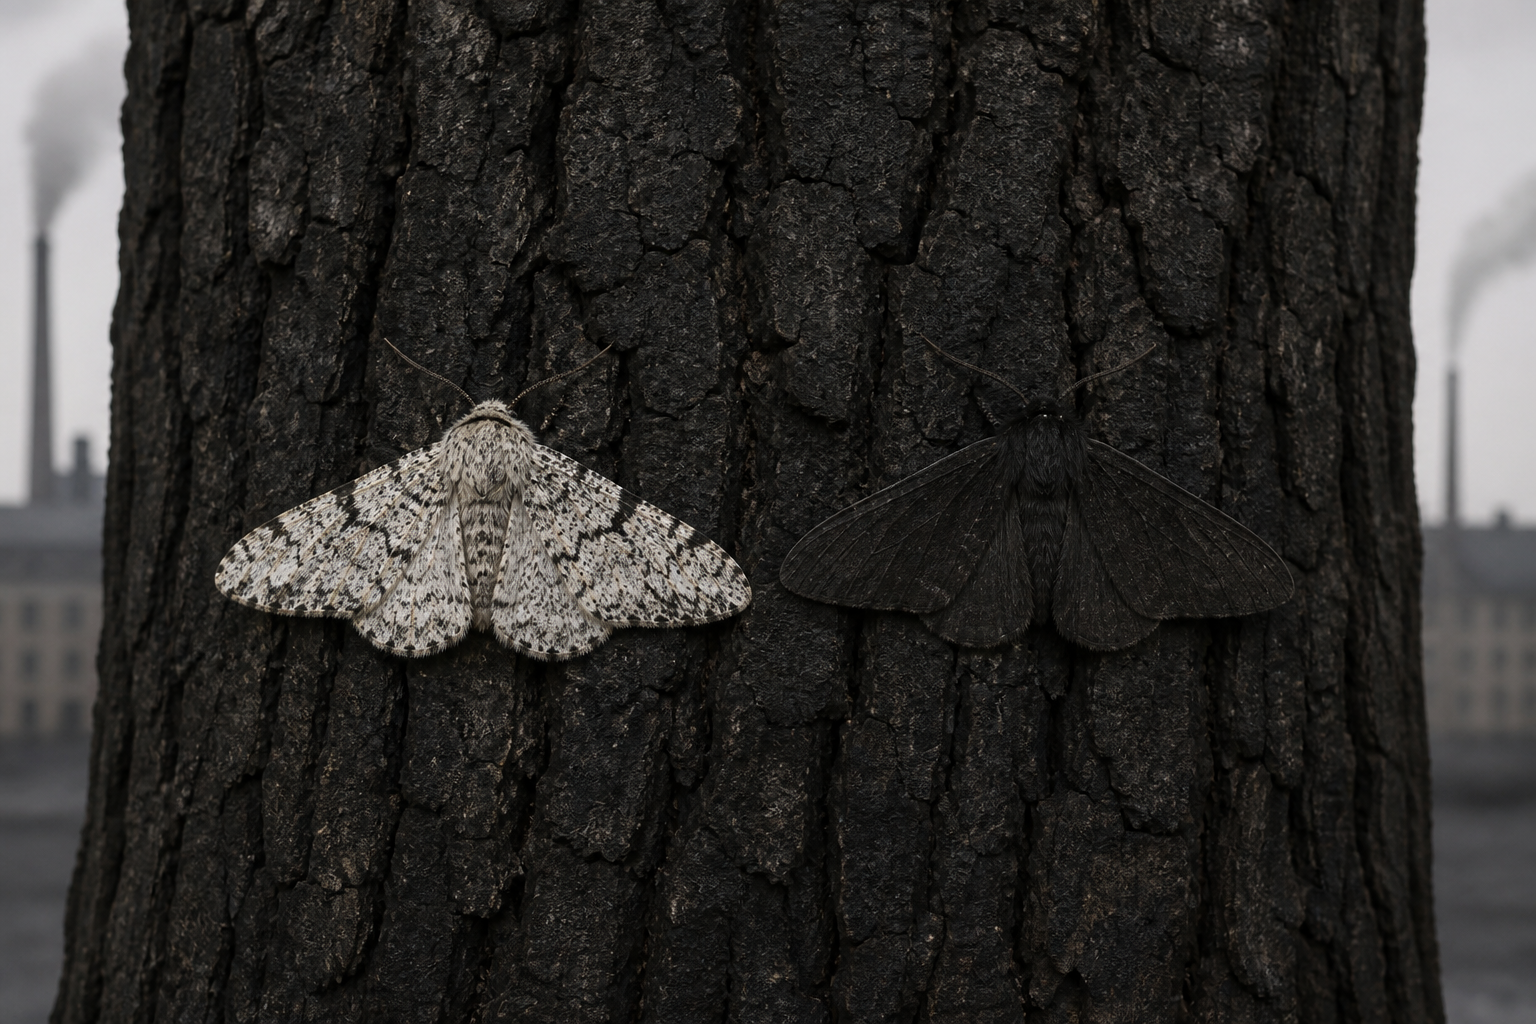
\includegraphics[width=0.6\linewidth]{images/book2/ai/g12-selection-peppered-moths.png}

{\small Dua bentuk ngengat lada pada batang yang menghitam oleh jelaga.
Burung berburu dengan penglihatan: pada kulit kayu ini bentuk pucat
yang diambil dan bentuk gelap selamat; pada batang bersih berlumut
kerak, sebaliknya.}
\end{omfigure}

\begin{example}[Seleksi oleh lawan jenis]\label{ex:g12:selection-drift-speciation:sexual}
Ekor merak jantan membuatnya lebih lambat dan lebih tampak oleh
pemangsa, namun ekor itu tetap bertahan karena merak betina memilih
jantan dengan ekor terbesar dan paling teratur: \omterm{def:g10:universal-dna:gene}{alel} yang memperbaiki
ekor lebih sering diwariskan, berapa pun ongkosnya bagi kelangsungan
hidup. \emph{Seleksi seksual} --- pemilihan pasangan --- menghasilkan
perhiasan, nyanyian dan pertarungan hewan, dan dapat mendorong sebuah
sifat ke arah yang tak akan pernah dipilih oleh kelangsungan hidup saja.
\end{example}

\section{Kebetulan: hanyutan genetik}

\begin{proposition}[Hanyutan genetik]\label{prop:g12:selection-drift-speciation:drift}
Dalam \omterm{def:g12:selection-drift-speciation:population}{populasi} mana pun yang berukuran terhingga, \omterm{def:g10:universal-dna:gene}{alel} satu generasi
adalah sampel acak dari generasi sebelumnya: individu mana yang
kebetulan berbiak, dan \omterm{def:g10:universal-dna:gene}{alel} mana yang kebetulan dibawa oleh gametnya,
berayun-ayun karena kebetulan. Karena itu \omterm{def:g12:selection-drift-speciation:population}{frekuensi alel} mengembara
dari satu generasi ke generasi berikutnya tanpa keuntungan apa pun
yang terlibat --- \emph{hanyutan genetik}\index{hanyutan genetik}.
Makin kecil \omterm{def:g12:selection-drift-speciation:population}{populasinya}, makin besar pengembaraannya; dalam \omterm{def:g12:selection-drift-speciation:population}{populasi}
kecil sebuah \omterm{def:g10:universal-dna:gene}{alel} dapat hilang, atau mencapai 100\%, semata-mata oleh
kebetulan dalam beberapa generasi, berapa pun nilainya.
\end{proposition}
\begin{proof}[Bukti percobaan]
\omterm{def:g12:selection-drift-speciation:population}{Populasi} yang didirikan oleh segelintir individu --- sebuah pulau yang
dikolonisasi oleh beberapa ekor burung, sebuah komunitas manusia
keturunan beberapa lusin pemukim --- membawa sampel yang terpelintir
dari \omterm{def:g10:universal-dna:gene}{alel} \omterm{def:g12:selection-drift-speciation:population}{populasi} asalnya: sebuah \omterm{def:g10:universal-dna:gene}{alel} penyakit langka dapat menjadi
umum di antara mereka, dan sebagian besar keragaman asalnya hilang.
\omterm{def:g10:biodiversity-scales:species}{Spesies} yang pernah melewati \emph{leher botol} berisi sangat sedikit
penyintas (citah pada \cref{ch:g10:biodiversity-scales}, anjing laut
gajah utara yang tersisa dua puluh ekor pada 1890) nyaris tidak
menunjukkan keragaman genetik hari ini, bahkan setelah pulih menjadi
ribuan. Dan di laboratorium, banyak \omterm{def:g12:selection-drift-speciation:population}{populasi} ulangan kecil yang mulai
pada frekuensi sama tersebar ke segala arah dalam beberapa generasi,
sedangkan \omterm{def:g12:selection-drift-speciation:population}{populasi} besar tetap di tempatnya.
\end{proof}

\begin{omfigure}
\begin{tikzpicture}
\begin{axis}[
  width=0.88\linewidth, height=5.8cm,
  axis x line=bottom, axis y line=left,
  xmin=0, xmax=20, ymin=0, ymax=1.05,
  xlabel={generasi}, ylabel={frekuensi alel $A$},
  xlabel style={font=\small, at={(axis description cs:0.5,-0.12)}, anchor=north},
  ylabel style={font=\small},
  tick label style={font=\small}, xtick={0,5,10,15,20}, ytick={0,0.25,0.5,0.75,1},
  legend style={at={(0.5,-0.3)}, anchor=north, legend columns=2, font=\small, draw=none},
]
\addplot[thick, omThm] coordinates {(0,0.5) (1,0.55) (2,0.6) (3,0.5) (4,0.65) (5,0.7) (6,0.6) (7,0.75) (8,0.85) (9,0.8) (10,0.9) (11,0.95) (12,1) (13,1) (14,1) (15,1) (16,1) (17,1) (18,1) (19,1) (20,1)};
\addplot[thick, omThm!60] coordinates {(0,0.5) (1,0.4) (2,0.45) (3,0.3) (4,0.35) (5,0.25) (6,0.3) (7,0.2) (8,0.1) (9,0.15) (10,0.05) (11,0.1) (12,0) (13,0) (14,0) (15,0) (16,0) (17,0) (18,0) (19,0) (20,0)};
\addplot[thick, omThm!35] coordinates {(0,0.5) (1,0.45) (2,0.55) (3,0.6) (4,0.5) (5,0.4) (6,0.45) (7,0.55) (8,0.6) (9,0.7) (10,0.65) (11,0.55) (12,0.5) (13,0.6) (14,0.65) (15,0.75) (16,0.7) (17,0.8) (18,0.75) (19,0.85) (20,0.8)};
\addplot[thick, omDef] coordinates {(0,0.5) (1,0.51) (2,0.49) (3,0.5) (4,0.52) (5,0.51) (6,0.5) (7,0.49) (8,0.48) (9,0.49) (10,0.5) (11,0.51) (12,0.52) (13,0.51) (14,0.5) (15,0.5) (16,0.49) (17,0.5) (18,0.51) (19,0.5) (20,0.5)};
\legend{tiga populasi 20 ekor, satu populasi 5000 ekor}
\end{axis}
\end{tikzpicture}

{\small Simulasi hanyutan sebuah \omterm{def:g10:universal-dna:gene}{alel} netral yang mulai pada 50\%.
Dalam \omterm{def:g12:selection-drift-speciation:population}{populasi} 20 individu \omterm{def:g10:universal-dna:gene}{alel} itu terpancang atau hilang dalam
belasan generasi, dengan arah berbeda setiap kali; dalam \omterm{def:g12:selection-drift-speciation:population}{populasi} 5000
\omterm{def:g10:universal-dna:gene}{alel} itu nyaris tidak bergerak.}
\end{omfigure}

\begin{example}[Sebuah efek pendiri]\label{ex:g12:selection-drift-speciation:founder}
Sebuah komunitas pulau didirikan oleh beberapa lusin pemukim, salah
seorangnya membawa \omterm{def:g10:universal-dna:gene}{alel} untuk kelainan \omterm{def:g11:the-eye:parts}{mata} yang langka. Sepuluh
generasi kemudian \omterm{def:g12:selection-drift-speciation:population}{frekuensi alel} itu di komunitas tersebut satu
berbanding sepuluh --- seratus kali nilai daratan utama --- karena satu
\omterm{def:g11:genes-and-disease:genetic}{pembawa} di antara tiga puluh pendiri sudah merupakan 1.7\% salinan, dan
hanyutan dalam \omterm{def:g12:selection-drift-speciation:population}{populasi} kecil yang terpencil mendorongnya lebih jauh.
\omterm{def:g10:universal-dna:gene}{Alel} itu tidak memberi keuntungan; kelimpahannya adalah kebetulan
tentang siapa yang naik perahu.
\end{example}

\begin{method}[Seleksi atau hanyutan?]\label{met:g12:selection-drift-speciation:which}
Menghadapi sebuah perubahan \omterm{def:g12:selection-drift-speciation:population}{frekuensi alel}:
\begin{enumerate}
  \item Perkirakan ukuran \omterm{def:g12:selection-drift-speciation:population}{populasinya}: hanyutan itu kuat di bawah
        beberapa ratus, dan dapat diabaikan pada jutaan.
  \item Cari arah yang mengikuti lingkungan (seleksi), atau jalan acak
        (hanyutan). \omterm{def:g12:selection-drift-speciation:population}{Populasi} ulangan yang bergerak searah menunjukkan
        seleksi; yang bergerak ke arah berbeda, hanyutan.
  \item Cari mekanisme yang menghubungkan \omterm{def:g10:universal-dna:gene}{alel} itu dengan kelangsungan
        hidup atau reproduksi; tanpa mekanisme itu, curigailah
        hanyutan.
  \item Ingatlah bahwa keduanya bekerja sekaligus: seleksi menetapkan
        kecenderungan, hanyutan menambahkan derau, dan dalam \omterm{def:g12:selection-drift-speciation:population}{populasi}
        kecil derau itu dapat menenggelamkan kecenderungannya.
\end{enumerate}
\end{method}

\section{Dari populasi menjadi spesies}

\begin{proposition}[Spesiasi]\label{prop:g12:selection-drift-speciation:speciation}
Dua \omterm{def:g12:selection-drift-speciation:population}{populasi} satu \omterm{def:g10:biodiversity-scales:species}{spesies} yang berhenti bertukar \omterm{def:g10:universal-dna:gene}{gen} --- terpisah oleh
penghalang geografi, perilaku atau waktu --- berevolusi terpisah:
masing-masing menghimpun \omterm{def:g11:mutations:mutation}{mutasinya} sendiri, diseleksi oleh
lingkungannya sendiri dan menghanyut menurut caranya sendiri. Ketika
perbedaannya sudah cukup jauh sehingga individu kedua \omterm{def:g12:selection-drift-speciation:population}{populasi} itu tak
lagi saling kawin, atau memberi keturunan yang mandul, bahkan ketika
bertemu lagi, ada dua \omterm{def:g10:biodiversity-scales:species}{spesies} di tempat yang tadinya satu.
\emph{Spesiasi}\index{spesiasi} adalah proses ini; biasanya perlu
ribuan hingga jutaan generasi, meskipun poliploidi
(\cref{ch:g12:diversification-of-life}) mencapainya dalam satu langkah.
\end{proposition}
\begin{proof}[Bukti percobaan]
Pulau: masing-masing pulau Galápagos memiliki burung finch tersendiri,
keturunan sebuah \omterm{def:g10:biodiversity-scales:species}{spesies} daratan dan paling mirip dengan burung finch
pulau tetangganya. Danau: satu ikan sikliid leluhur telah memberi
ratusan \omterm{def:g10:biodiversity-scales:species}{spesies} dalam satu danau Afrika dalam beberapa ratus ribu
tahun, terpisah oleh habitat dan oleh pilihan betina atas warna
jantan. \omterm{def:g10:biodiversity-scales:species}{Spesies} cincin: \omterm{def:g12:selection-drift-speciation:population}{populasi} seekor camar menyebar mengelilingi
Arktik, saling kawin dengan tetangganya sepanjang lingkaran, sampai
kedua ujungnya bertemu di Eropa sebagai bentuk yang tidak saling kawin
--- sebuah batas \omterm{def:g10:biodiversity-scales:species}{spesies} yang tertangkap sedang terbentuk. Dan \omterm{def:g10:biodiversity-scales:species}{spesies}
yang baru saja terpisah, seperti beruang kutub dan beruang cokelat,
masih sesekali menghasilkan hibrida yang subur: batas itu soal derajat.
\end{proof}

\begin{omfigure}
\begin{tikzpicture}[font=\small, >=Stealth]
  % one population
  \draw[thick, fill=omDef!12] (0,0) ellipse (1.4 and 0.8);
  \node at (0,0) {satu populasi};
  \draw[->, thick] (1.6,0) -- (2.6,0) node[midway, above, font=\scriptsize, align=center] {penghalang\\ muncul};
  % two separated
  \draw[thick, fill=omDef!12] (4.0,0.9) ellipse (1.2 and 0.6); \node at (4.0,0.9) {populasi 1};
  \draw[thick, fill=omDef!12] (4.0,-0.9) ellipse (1.2 and 0.6); \node at (4.0,-0.9) {populasi 2};
  \draw[very thick, gray] (2.7,0) -- (5.3,0);
  \draw[->, thick] (5.5,0) -- (6.5,0) node[midway, above, font=\scriptsize, align=center] {evolusi\\ terpisah};
  % diverged
  \draw[thick, fill=omMeth!15] (7.9,0.9) ellipse (1.2 and 0.6); \node at (7.9,0.9) {mutasi 1};
  \draw[thick, fill=omThm!15] (7.9,-0.9) ellipse (1.2 and 0.6); \node at (7.9,-0.9) {mutasi 2};
  \node[font=\scriptsize, align=center] at (7.9,0.0) {seleksi sendiri,\\ hanyutan sendiri};
  \draw[->, thick] (9.3,0) -- (10.3,0) node[midway, above, font=\scriptsize, align=center] {penghalang\\ hilang};
  % two species
  \draw[thick, fill=omMeth!15] (11.6,0.7) ellipse (1.1 and 0.55); \node at (11.6,0.7) {spesies 1};
  \draw[thick, fill=omThm!15] (11.6,-0.7) ellipse (1.1 and 0.55); \node at (11.6,-0.7) {spesies 2};
  \node[font=\scriptsize, align=center] at (11.6,0.0) {tidak saling kawin};
\end{tikzpicture}

{\small \omterm{prop:g12:selection-drift-speciation:speciation}{Spesiasi} oleh pemisahan. Sebuah penghalang membelah \omterm{def:g12:selection-drift-speciation:population}{populasi};
setiap belahan berevolusi sendiri; ketika keduanya bertemu lagi,
mereka tak lagi saling kawin. Penghalang itu dapat berupa selat,
gunung, perubahan habitat, atau pilihan dalam perkawinan.}
\end{omfigure}

\begin{proposition}[Spesies, ditimbang ulang]\label{prop:g12:selection-drift-speciation:concept}
Sebuah \omterm{def:g10:biodiversity-scales:species}{spesies} adalah satu \omterm{def:g12:selection-drift-speciation:population}{populasi}, atau sehimpunan \omterm{def:g12:selection-drift-speciation:population}{populasi}, yang
anggotanya saling kawin di antara mereka sendiri dan terisolasi secara
genetik dari himpunan lain semacam itu --- definisi yang berlaku bagi
kebanyakan hewan dan tumbuhan pada suatu saat tertentu, tetapi punya
tepi: \omterm{def:g12:selection-drift-speciation:population}{populasi} yang sedang memisah, \omterm{def:g10:biodiversity-scales:species}{spesies} yang masih berhibrida,
organisme yang berbiak tanpa seks. \omterm{def:g10:biodiversity-scales:species}{Spesies} bukanlah tipe yang tetap
melainkan sebuah garis keturunan dalam waktu: ia mulai ketika sebuah
\omterm{def:g12:selection-drift-speciation:population}{populasi} terisolasi, ada selama anggotanya terus saling kawin, dan
berakhir oleh kepunahan atau oleh pembelahan menjadi \omterm{def:g10:biodiversity-scales:species}{spesies} baru.
\omterm{def:g10:biodiversity-scales:species}{Spesies} yang hidup hari ini adalah ujung-ujung sebuah pohon yang
cabangnya menjadi pokok bahasan \cref{ch:g12:phylogenetic-trees}.
\end{proposition}
\admitted

\begin{remark}[Evolusi, dirakit]\label{rem:g12:selection-drift-speciation:assembled}
\omterm{def:g11:mutations:mutation}{Mutasi} dan pengocokan memasok keragaman; duplikasi, transfer,
poliploidi, pengaturan dan \omterm{def:g12:diversification-of-life:symbiosis}{simbiosis} memasok lebih banyak lagi;
seleksi memilahnya menurut lingkungan, hanyutan menurut kebetulan;
isolasi membiarkan \omterm{def:g12:selection-drift-speciation:population}{populasi} memencar sampai menjadi \omterm{def:g10:biodiversity-scales:species}{spesies}; kepunahan
menyingkirkannya. Tidak satu pun langkah ini punya tujuan, dan tidak
satu pun menatap ke depan; bersama-sama, sepanjang empat miliar tahun
rekaman fosil, semuanya telah menghasilkan keanekaragaman
\cref{ch:g10:biodiversity-scales}. Teori yang menyebutkan
langkah-langkah ini dan interaksinya adalah teori evolusi, dan setiap
bab tahun ini telah menjadi sekeping buktinya.
\end{remark}

\section{Latihan}

\begin{exercise}[$\star$]\label{exo:g12:selection-drift-speciation:1}
Definisikan \omterm{def:g12:selection-drift-speciation:population}{frekuensi alel}, dan berikan perbandingan \omterm{def:g11:enzymes-and-phenotype:phenotype}{genotipe} sebuah
\omterm{def:g12:selection-drift-speciation:population}{populasi} pada keadaan acuan dengan $p = 0.8$.
\end{exercise}

\begin{exercise}[$\star$]\label{exo:g12:selection-drift-speciation:2}
Definisikan \omterm{def:g12:selection-drift-speciation:selection}{seleksi alam} dan \omterm{prop:g12:selection-drift-speciation:drift}{hanyutan genetik}, lalu nyatakan perbedaan
hakiki di antara keduanya.
\end{exercise}

\begin{exercise}[$\star$]\label{exo:g12:selection-drift-speciation:3}
Dari gambar ngengat, bacalah frekuensi bentuk gelap pada 1880 dan pada
1980, dan sebutkan perubahan lingkungan di balik masing-masingnya.
\end{exercise}

\begin{exercise}[$\star$]\label{exo:g12:selection-drift-speciation:4}
Mengapa hanyutan lebih berpengaruh di dalam \omterm{def:g12:selection-drift-speciation:population}{populasi} kecil?
\end{exercise}

\begin{exercise}[$\star$]\label{exo:g12:selection-drift-speciation:5}
Apa yang diperlukan agar satu \omterm{def:g12:selection-drift-speciation:population}{populasi} menjadi dua \omterm{def:g10:biodiversity-scales:species}{spesies}?
\end{exercise}

\begin{exercise}[$\star\star$]\label{exo:g12:selection-drift-speciation:6}
Dalam \omterm{def:g12:selection-drift-speciation:population}{populasi} 500 ekor, 320 bergenotipe $AA$, 160 $Aa$ dan 20 $aa$. Hitunglah
$p$ dan $q$, lalu cacah \omterm{def:g11:enzymes-and-phenotype:phenotype}{genotipe} yang diharapkan pada keadaan acuan,
dan bandingkan keduanya.
\end{exercise}

\begin{exercise}[$\star\star$]\label{exo:g12:selection-drift-speciation:7}
Sebuah \omterm{def:g10:universal-dna:gene}{alel} \omterm{def:g11:genes-and-disease:genetic}{resesif} berfrekuensi 0.01. Berapa bagian \omterm{def:g12:selection-drift-speciation:population}{populasi} yang
menampakkan sifat \omterm{def:g11:genes-and-disease:genetic}{resesif} itu, dan berapa bagian yang membawa \omterm{def:g10:universal-dna:gene}{alel} itu
tanpa terlihat? Mengapa \omterm{def:g10:universal-dna:gene}{alel} itu begitu sulit dilenyapkan oleh seleksi
terhadap sifatnya?
\end{exercise}

\begin{exercise}[$\star\star$]\label{exo:g12:selection-drift-speciation:8}
Dari gambar hanyutan, dalam berapa generasi \omterm{def:g10:universal-dna:gene}{alel} itu terpancang atau
hilang pada dua \omterm{def:g12:selection-drift-speciation:population}{populasi} kecil yang mencapai ujung? Mengapa yang
ketiga tidak?
\end{exercise}

\begin{exercise}[$\star\star$]\label{exo:g12:selection-drift-speciation:9}
Jelaskan mengapa \omterm{def:g10:universal-dna:gene}{alel} gelap ngengat lada tidak mencapai 100\% selama
dasawarsa berjelaga, dengan memakai ngengat yang hidup dan berbiak di
pedesaan.
\end{exercise}

\begin{exercise}[$\star\star$]\label{exo:g12:selection-drift-speciation:10}
Dua puluh anjing laut selamat dari sebuah leher botol; \omterm{def:g10:biodiversity-scales:species}{spesies} itu
kini berjumlah 100\,000 ekor tetapi nyaris tanpa keragaman genetik.
Jelaskan dengan hanyutan.
\end{exercise}

\begin{exercise}[$\star\star$]\label{exo:g12:selection-drift-speciation:11}
Terapkan \cref{met:g12:selection-drift-speciation:which} pada dua
kasus: sebuah \omterm{def:g10:universal-dna:gene}{alel} yang naik di sepuluh \omterm{def:g12:selection-drift-speciation:population}{populasi} danau terpisah
sekaligus setelah pemangsa baru datang; dan sebuah \omterm{def:g10:universal-dna:gene}{alel} yang mencapai
80\% pada satu \omterm{def:g12:selection-drift-speciation:population}{populasi} pulau berisi tiga puluh ekor burung.
\end{exercise}

\begin{exercise}[$\star\star\star$]\label{exo:g12:selection-drift-speciation:12}
Di sebuah wilayah bermalaria, \omterm{def:g10:universal-dna:gene}{alel} sabit berfrekuensi 0.15
walaupun anak $aa$ jarang bertahan hidup. Dengan memakai perbandingan
\omterm{def:g11:enzymes-and-phenotype:phenotype}{genotipe}, hitunglah bagian bayi baru lahir yang $AA$, $Aa$ dan $aa$,
lalu jelaskan bagaimana keuntungan $Aa$ terhadap malaria menjaga \omterm{def:g10:universal-dna:gene}{alel}
itu tetap umum meskipun ada kehilangan $aa$.
\end{exercise}

\begin{exercise}[$\star\star\star$]\label{exo:g12:selection-drift-speciation:13}
Dua \omterm{def:g10:biodiversity-scales:species}{spesies} sikliid dalam satu danau berbeda terutama pada warna
jantannya, dan betina masing-masing memilih warnanya sendiri. Dalam
air keruh, tempat warna tak dapat terlihat, keduanya berhibrida dengan
bebas. Apa yang mengisolasi kedua \omterm{def:g10:biodiversity-scales:species}{spesies} itu, dan apa yang dikatakan
kasus air keruh tentang seberapa baru pemisahannya?
\end{exercise}

\begin{exercise}[$\star\star\star$]\label{exo:g12:selection-drift-speciation:14}
Jelaskan mengapa \omterm{def:g10:biodiversity-scales:species}{spesies} cincin camar merupakan alasan bahwa spesiasi
berlangsung berangsur, dan mengapa kedua ujung yang bertemu di Eropa
tetap disebut dua \omterm{def:g10:biodiversity-scales:species}{spesies}.
\end{exercise}

\begin{exercise}[$\star\star\star$]\label{exo:g12:selection-drift-speciation:15}
``Seleksi membuat organisme menjadi lebih baik.'' Bahaslah dalam satu
paragraf: lebih baik dalam hal apa, di mana, dan dibandingkan dengan
siapa; lalu apa yang ditambahkan oleh hanyutan, pembalikan dan seleksi
seksual.
\end{exercise}

\section{Soal: Tikus-Tikus di Sebuah Pulau}

\begin{problem}[{Soal akhir pekan --- sebuah populasi tikus di pulau:
frekuensi alelnya dihitung, seleksi oleh pemangsa baru diikuti,
hanyutan sebuah koloni mungil disimulasikan, dan kelahiran sebuah
spesies diramalkan}]
\label{pb:g12:selection-drift-speciation:1}
Di sebuah pulau berbatu, tikus membawa \omterm{def:g10:universal-dna:gene}{gen} warna bulu dengan dua \omterm{def:g10:universal-dna:gene}{alel}: $D$
(gelap, \omterm{def:g11:genes-and-disease:genetic}{dominan}) dan $d$ (pucat). Sensus atas 2000 tikus menemukan 720 tikus
gelap bergenotipe $DD$, 960 gelap $Dd$, dan 320 pucat $dd$.

\medskip
\noindent\textbf{Bagian I --- \omterm{def:g12:selection-drift-speciation:population}{Populasi} saat ini.}
\begin{enumerate}
  \item Hitunglah frekuensi $p$ dari $D$ dan $q$ dari $d$ dengan
        mencacah salinannya.
  \item Hitunglah cacah \omterm{def:g11:enzymes-and-phenotype:phenotype}{genotipe} yang diharapkan pada keadaan acuan
        lalu bandingkan dengan sensus. Apakah \omterm{def:g12:selection-drift-speciation:population}{populasi} itu berada pada
        keadaan acuan?
  \item Berapa bagian tikus gelap yang merupakan \omterm{def:g11:genes-and-disease:genetic}{pembawa} $d$?
  \item Jelaskan, dari jawaban sebelumnya, mengapa menyingkirkan semua
        tikus pucat dari pulau itu selama satu generasi hanya akan
        menurunkan $q$ sedikit saja. Hitunglah $q$ yang baru setelah
        penyingkiran itu, jika tikus yang tersisa berbiak secara acak.
  \item Syarat mana di antara empat syarat keadaan acuan yang paling
        mungkin gagal di sebuah pulau kecil, dan dengan akibat apa?
\end{enumerate}

\medskip
\noindent\textbf{Bagian II --- Seekor pemangsa datang.}
Burung hantu mengolonisasi pulau itu. Di atas batu yang pucat, tikus
gelap terlihat dan dimangsa dua kali lebih sering: setiap generasi,
separuh tikus gelap mati sebelum berbiak sedangkan semua tikus pucat
selamat.
\begin{enumerate}[resume]
  \item Mulai dari angka sensus, hitunglah cacah tikus setiap \omterm{def:g11:enzymes-and-phenotype:phenotype}{genotipe}
        yang bertahan hidup untuk berbiak pada generasi pertama.
  \item Hitunglah $p$ dan $q$ di antara para penyintasnya.
  \item Jika para penyintas kawin secara acak, hitunglah perbandingan
        \omterm{def:g11:enzymes-and-phenotype:phenotype}{genotipe} generasi berikutnya, lalu terapkan burung hantu itu
        lagi dan hitunglah $q$ di antara penyintasnya.
  \item Ulangi sekali lagi (dua angka penting). Uraikan kecenderungan
        $q$ sepanjang ketiga generasi itu.
  \item Jelaskan mengapa $q$ naik terus, dan mengapa $D$, tak seperti
        \omterm{def:g10:universal-dna:gene}{alel} \omterm{def:g11:genes-and-disease:genetic}{resesif} di bawah seleksi yang sama, dapat dilenyapkan
        sepenuhnya.
\end{enumerate}

\medskip
\noindent\textbf{Bagian III --- Sebuah koloni berisi enam ekor.}
Sebuah badai membawa enam tikus ke pulau kecil tetangga: 2 $DD$, 3 $Dd$, 1 $dd$.
\begin{enumerate}[resume]
  \item Hitunglah $q$ di koloni itu dan bandingkan dengan pulau besar.
  \item Pada anakan pertama, secara kebetulan, hanya kedua $DD$ dan
        satu $Dd$ yang berbiak. Berapa saja nilai $q$ yang mungkin pada
        generasi berikutnya? Apa yang terjadi pada keragaman \omterm{def:g12:selection-drift-speciation:population}{populasi}?
  \item Jelaskan mengapa, di pulau kecil itu, sebuah \omterm{def:g10:universal-dna:gene}{alel} dapat lenyap
        dalam beberapa generasi tanpa burung hantu atau keuntungan apa
        pun.
  \item Pulau kecil itu tak berburung hantu. Ramalkan nasib $d$ di
        sana, lalu katakan mengapa dua pulau bertetangga dapat berakhir
        dengan warna bulu berbeda tanpa alasan adaptasi apa pun.
  \item Sebutkan nama prosesnya, dan ciri koloni itu yang membuatnya
        \omterm{def:g11:genes-and-disease:genetic}{dominan} di sana.
\end{enumerate}

\medskip
\noindent\textbf{Bagian IV --- Sepuluh ribu tahun kemudian.}
Tikus pulau kecil itu, dalam keterpencilannya, telah memencar: lebih
kecil, lebih pucat, berbiak pada musim yang berbeda. Ketika disatukan
dengan tikus pulau besar di laboratorium, keduanya jarang kawin, dan
sedikit hibrida yang ada mandul.
\begin{enumerate}[resume]
  \item Apakah tikus pulau kecil itu \omterm{def:g10:biodiversity-scales:species}{spesies} baru? Berikan alasannya
        dengan definisi tadi.
  \item Sebutkan penghalang yang memulai prosesnya dan dua mekanisme
        yang mendorong pemencarannya.
  \item Musim berbiak keduanya berbeda. Jelaskan bagaimana perbedaan
        semacam itu, sekali hadir, memperkuat isolasinya.
  \item Jika pulau kecil itu bersambung lagi dengan pulau besar besok,
        apakah keduanya akan melebur kembali menjadi satu \omterm{def:g12:selection-drift-speciation:population}{populasi}?
        Bedakan kasus pertanyaan 17 dari tahap yang lebih awal,
        katakanlah setelah 100 tahun.
  \item Nyatakan hasilnya: frekuensi $d$ di pulau besar sebelum dan
        sesudah tiga generasi burung hantu, nasib $d$ di pulau kecil
        dan proses yang bertanggung jawab, serta jumlah \omterm{def:g10:biodiversity-scales:species}{spesies} pada
        akhirnya.
\end{enumerate}
\end{problem}
